% ============================================================
% EMA AI — Owner Requirements Report
% Logic, Evidence, Scoring, and Review Framework
% Customer-Facing Technical Document
% ============================================================
% Build: pdflatex -interaction=nonstopmode ema_ai_owner_requirements_logic_framework.tex (×3)
% ============================================================
\documentclass[10pt,letterpaper]{article}

% ------------------------------------------------------------
% Packages
% ------------------------------------------------------------
\usepackage[margin=0.58in]{geometry}
\usepackage[T1]{fontenc}
\usepackage[utf8]{inputenc}
\usepackage{lmodern}
\usepackage{microtype}
\usepackage{xcolor}
\usepackage{array}
\usepackage{tabularx}
\usepackage{booktabs}
\usepackage{enumitem}
\usepackage[most]{tcolorbox}
\usepackage{fancyhdr}
\usepackage{lastpage}
\usepackage{hyperref}
\usepackage{titlesec}
\usepackage{colortbl}
\usepackage{tikz}
\usetikzlibrary{shapes.geometric}
\usepackage{longtable}
\usepackage{amsmath}
\usepackage{ragged2e}
\usepackage{caption}

% ------------------------------------------------------------
% Page setup
% ------------------------------------------------------------
\pagestyle{fancy}
\fancyhf{}
\renewcommand{\headrulewidth}{0pt}
\fancyfoot[L]{\footnotesize EMA AI --- Owner Requirements Logic Framework}
\fancyfoot[C]{\footnotesize}
\fancyfoot[R]{\footnotesize Page \thepage\ of \pageref{LastPage}}

\hypersetup{colorlinks=true,linkcolor=emaNavy,urlcolor=emaNavy,citecolor=emaNavy}

% ------------------------------------------------------------
% Color palette
% ------------------------------------------------------------
\definecolor{emaBlue}{HTML}{2563EB}
\definecolor{emaBlueDark}{HTML}{1D4ED8}
\definecolor{emaNavy}{HTML}{0F172A}
\definecolor{emaSlate}{HTML}{334155}
\definecolor{emaText}{HTML}{1E293B}
\definecolor{emaMuted}{HTML}{64748B}
\definecolor{emaLine}{HTML}{E2E8F0}
\definecolor{emaSoft}{HTML}{F8FAFC}
\definecolor{emaSoft2}{HTML}{F1F5F9}
\definecolor{emaGreen}{HTML}{15803D}
\definecolor{emaGreenBg}{HTML}{DCFCE7}
\definecolor{emaRed}{HTML}{B91C1C}
\definecolor{emaRedBg}{HTML}{FEE2E2}
\definecolor{emaAmber}{HTML}{B45309}
\definecolor{emaAmberBg}{HTML}{FEF3C7}
\definecolor{emaPurple}{HTML}{6D28D9}
\definecolor{emaPurpleBg}{HTML}{EDE9FE}
\definecolor{emaGrayBg}{HTML}{F1F5F9}
\definecolor{guardrailBlue}{HTML}{EFF6FF}
\definecolor{guardrailBorder}{HTML}{BFDBFE}

% Semantic status colors
\newcommand{\colMet}{\color{emaGreen}}
\newcommand{\colNotMet}{\color{emaRed}}
\newcommand{\colReview}{\color{emaAmber}}
\newcommand{\colInsuff}{\color{emaPurple}}
\newcommand{\colNA}{\color{emaSlate}}

% ------------------------------------------------------------
% Global style
% ------------------------------------------------------------
\renewcommand{\familydefault}{\sfdefault}
\setlength{\parindent}{0pt}
\setlength{\parskip}{5pt}
\setlist[itemize]{leftmargin=1.15em,itemsep=2pt,topsep=2pt}
\setlist[enumerate]{leftmargin=1.35em,itemsep=2pt,topsep=2pt}

\titleformat{\section}{\Large\bfseries\color{emaNavy}}{}{0em}{}
\titlespacing{\section}{0pt}{16pt}{6pt}
\titleformat{\subsection}{\normalsize\bfseries\color{emaNavy}}{}{0em}{}
\titlespacing{\subsection}{0pt}{10pt}{4pt}
\titleformat{\subsubsection}{\small\bfseries\color{emaSlate}}{}{0em}{}
\titlespacing{\subsubsection}{0pt}{8pt}{3pt}

\tcbset{enhanced,boxrule=0.6pt,arc=3mm,left=8pt,right=8pt,top=7pt,bottom=7pt,
        colback=white,colframe=emaLine,breakable}

\widowpenalty=10000
\clubpenalty=10000

% ------------------------------------------------------------
% Custom commands
% ------------------------------------------------------------
\newcommand{\muted}[1]{\textcolor{emaMuted}{#1}}
\newcommand{\strong}[1]{\textbf{\textcolor{emaNavy}{#1}}}
\newcommand{\smalllabel}[1]{{\scriptsize\textcolor{emaMuted}{\MakeUppercase{#1}}}}
\newcommand{\code}[1]{\texttt{#1}}

% Status badges
\newcommand{\badge}[3]{\tcbox[on line,colback=#2,colframe=#2,boxrule=0pt,
    arc=2mm,left=5pt,right=5pt,top=2pt,bottom=2pt]{\scriptsize\textbf{\textcolor{#3}{#1}}}}
\newcommand{\metbadge}{\badge{Met}{emaGreenBg}{emaGreen}}
\newcommand{\notmetbadge}{\badge{Not Met}{emaRedBg}{emaRed}}
\newcommand{\reviewbadge}{\badge{Needs Human Review}{emaAmberBg}{emaAmber}}
\newcommand{\insufficientbadge}{\badge{Insufficient Model Data}{emaPurpleBg}{emaPurple}}
\newcommand{\nabadge}{\badge{Not Applicable}{emaGrayBg}{emaSlate}}

% Guardrail callout
\newcommand{\guardrailbox}[1]{%
\begin{tcolorbox}[colback=guardrailBlue,colframe=guardrailBorder,
    boxrule=0.6pt,arc=2mm,left=10pt,right=10pt,top=8pt,bottom=8pt]\small #1%
\end{tcolorbox}}

% Key concept callout (border-left style)
\newcommand{\keyconcept}[1]{%
\begin{tcolorbox}[colback=emaSoft,borderline west={3pt}{0pt}{emaBlue}]\small #1%
\end{tcolorbox}}

% Flow arrow
\newcommand{\flowarrow}{\ensuremath{\;\boldsymbol{\rightarrow}\;}}

% ------------------------------------------------------------
% TikZ styles (global, not deprecated \tikzstyle)
% ------------------------------------------------------------
\tikzset{
  block/.style={rectangle,draw=emaNavy!60,fill=emaSoft,
    minimum width=2.8cm,minimum height=0.7cm,align=center,font=\footnotesize},
  arrow/.style={->,>=stealth,thick},
  decision/.style={diamond,draw=emaAmber!60,fill=emaAmberBg,
    minimum width=2.2cm,minimum height=0.7cm,align=center,font=\footnotesize},
  result/.style={rectangle,draw=emaGreen!60,fill=emaGreenBg,
    minimum width=2.8cm,minimum height=0.7cm,align=center,font=\footnotesize},
  etype/.style={rectangle,draw=emaNavy!60,fill=emaSoft,
    minimum width=2.8cm,minimum height=0.7cm,align=center,font=\footnotesize},
  eclass/.style={rectangle,draw=emaBlue!60,fill=guardrailBlue,
    minimum width=2.8cm,minimum height=0.7cm,align=center,font=\footnotesize},
  loopblock/.style={rectangle,draw=emaNavy!60,fill=emaSoft,
    minimum width=2.8cm,minimum height=0.7cm,align=center,font=\footnotesize},
  flowstyle/.style={font=\footnotesize}
}

% ------------------------------------------------------------
% Document
% ------------------------------------------------------------
\begin{document}
\color{emaText}

% ============================================================
% Cover Page
% ============================================================
\thispagestyle{empty}
\begin{tcolorbox}[colback=white,colframe=emaNavy,boxrule=1.5pt,arc=5mm,
    left=20pt,right=20pt,top=28pt,bottom=28pt]
\begin{center}
  \vspace{6pt}
  {\Huge\bfseries\textcolor{emaNavy}{EMA AI}}\\[2pt]
  {\Huge\bfseries\textcolor{emaNavy}{Owner Requirements Report}}\\[10pt]
  {\Large\textcolor{emaMuted}{Logic, Evidence, Scoring, and Review Framework}}\\[20pt]
  {\normalsize\textcolor{emaSlate}{MVP --- Customer-Facing Technical Document}}\\[4pt]
  {\normalsize\textcolor{emaSlate}{June 2026}}\\[20pt]
  \begin{tcolorbox}[colback=emaSoft,colframe=emaLine,boxrule=0.5pt,arc=2mm,
      left=14pt,right=14pt,top=8pt,bottom=8pt]
    {\small\itshape\textcolor{emaMuted}{Prepared for discussion and technical validation.%
        \ Not a final compliance certification.}}
  \end{tcolorbox}
  \vspace{10pt}
  {\footnotesize\textcolor{emaMuted}{EMA AI --- Engineering Intelligence / Deliverable Readiness Platform}}\\[2pt]
  {\footnotesize\textcolor{emaMuted}{Revit Export $\rightarrow$ FastAPI $\rightarrow$ PostgreSQL $\rightarrow$%
      \ QA/QC $\rightarrow$ Owner Requirements $\rightarrow$ Evidence $\rightarrow$%
      \ Readiness $\rightarrow$ Dashboard}}
  \vspace{6pt}
\end{center}
\end{tcolorbox}

\vfill
\begin{tcolorbox}[colback=emaSoft2,colframe=emaLine,arc=2mm]
\small\textcolor{emaSlate}{\textbf{Document purpose:} This document describes the complete structure,
  logic, evidence model, scoring framework, and review methodology underlying the EMA AI Owner
  Requirements Report. It is intended for EMA leadership, BIM/VDC managers, engineering discipline
  leads, technical reviewers, and the delivery team. All descriptions reflect the current MVP
  implementation as of June 2026.}
\end{tcolorbox}
\newpage

% ============================================================
% Table of Contents
% ============================================================
\tableofcontents
\newpage

% ============================================================
% 1. Executive Summary
% ============================================================
\section{Executive Summary}

The EMA AI Owner Requirements Report is a structured first-pass evidence review generated from
synced Revit model data, owner requirement workbooks, and deterministic classification logic. It
produces a traceable, auditable mapping from each client-supplied requirement to the available model
evidence, an evaluated status, a prioritisation score, and a recommended next action.

\strong{What the report delivers:}
\begin{itemize}
  \item Normalises raw owner requirement rows from Excel workbooks into structured, queryable records.
  \item Classifies each requirement by discipline, validation type, and required evidence category.
  \item Evaluates available Revit model evidence using deterministic pattern matching and parameter
        validation.
  \item Assigns a status (\textsc{Met}, \textsc{Not Met}, \textsc{Needs Human Review},
        \textsc{Insufficient Model Data}, \textsc{Not Applicable}) based on evidence quality and
        completeness.
  \item Computes a Key Issue Score for prioritisation across requirements, disciplines, and
        deliverables.
  \item Generates Next Best Action guidance for each requirement.
  \item Aggregates to a project-level Readiness Score weighted across requirement coverage, QA/QC
        health, and sync freshness.
\end{itemize}

\strong{What the report does not do:}
\begin{itemize}
  \item It does not certify code compliance, contract compliance, or professional engineering
        approval.
  \item It does not replace licensed engineering review.
  \item It does not treat generic model element presence as proof of requirement satisfaction.
  \item It does not automatically close specification, drawing, or manual requirements without human
        review.
  \item It does not produce a final compliance certificate.
\end{itemize}

\strong{Why traceability matters:} Every requirement retains its source workbook, worksheet row,
discipline, category, evidence lineage, scoring breakdown, and review history. This enables
reviewers to trace any status decision back to the original evidence and rule logic.

\strong{Why human-in-the-loop review is required:} Revit model evidence alone is insufficient for
many requirement types. Specification requirements, manufacturer standards, control sequences,
termination details, and coordination items require professional engineering judgment. The report
clearly separates what the system can evaluate from what must be reviewed by a qualified
professional.

\guardrailbox{\strong{Core positioning:} EMA AI does not replace engineering judgment. It provides a
  structured first-pass evidence review that helps identify what appears supported by available model
  or export evidence; what appears missing or conflicting; what requires human review; what cannot
  be safely evaluated from current data; and what discipline action should happen next.}

% ============================================================
% 2. Report Purpose
% ============================================================
\section{Report Purpose}

The Owner Requirements Report serves as a structured review layer between raw owner requirements and
engineering deliverable readiness. The pipeline follows a deterministic chain:

\[
\begin{aligned}
&\text{Owner Requirements} \flowarrow \text{Requirement Type} \flowarrow \text{Expected Evidence}\\
&\flowarrow \text{Available Evidence} \flowarrow \text{Status} \flowarrow \text{Key Issue Score}\\
&\flowarrow \text{Next Best Action}
\end{aligned}
\]

Each step is deterministic, traceable, and auditable. The system does not generate statuses from
opaque models. Every status decision can be traced to specific evidence rows, parameter matches,
rule codes, and classification logic.

\keyconcept{\strong{Design principle:} The report is conservative by design. When evidence is
  ambiguous, missing, or insufficient, the system escalates to human review rather than guessing a
  status. This reduces false positive Met assignments and ensures that every reported status has a
  defensible evidence basis.}

% ============================================================
% 3. Source Inputs
% ============================================================
\section{Source Inputs}

The report draws on the following source input categories:

\begin{longtable}{p{1.5in}p{1.2in}p{3.8in}}
\caption{Source inputs and their roles in the evidence pipeline}
\label{tab:source-inputs}\\
\toprule
\textbf{Source} & \textbf{Role} & \textbf{Description} \\
\midrule
\endhead
Owner Requirements Workbook / Excel & Authoritative & Client-supplied XLSX containing requirement
  rows, discipline mapping, categories, and optional status fields. Ingested by the requirement
  loader. \\
\hline
Revit Model Export JSON & Authoritative & JSON export from EMA Revit add-in containing elements,
  categories, families, types, instance and type parameters, levels, and discipline metadata. The
  source of truth for model evidence. \\
\hline
Element / Category / Family / Type Data & Supporting & Individual element records from the export,
  classified by category, family name, type name, and unique ID. Used for evidence candidate
  matching. \\
\hline
Instance / Type Parameters & Supporting & Parameter key-value pairs on each element (e.g., Panel,
  Circuit Number, Voltage, Load, Mark, System Name). Used for direct evidence validation. \\
\hline
Discipline Metadata & Supporting & Discipline labels derived from workbook worksheet context, source
  file conventions, or keyword inference. \\
\hline
Evidence Records & Supporting & \texttt{RequirementEvidence} table entries linking requirements to
  model elements, sheets, spec sections, or manual entries. Each record carries an evidence type,
  evidence status, and review status. \\
\hline
Report Hidden JSON Context & Supporting & Inline JSON embedded in HTML reports containing full
  report metadata, requirement rows, evidence rows, element references, rule applications, summary
  metrics, and issue scores. \\
\bottomrule
\end{longtable}

\strong{Authoritative vs.\ supporting distinction:} Authoritative sources drive primary status
decisions. Supporting sources provide context, evidence candidates, and audit trail information but
cannot independently change a status.

% ============================================================
% 4. Requirement Normalization
% ============================================================
\section{Requirement Normalization}

Raw requirement rows from Excel workbooks undergo structured normalisation before classification and
evidence evaluation. Each field is mapped from its raw workbook representation to a normalised
internal schema.

\begin{longtable}{p{1.4in}p{1.5in}p{1.4in}p{1.5in}}
\caption{Raw-to-normalised field mapping with examples\label{tab:normalization}}\\
\toprule
\textbf{Raw Field} & \textbf{Normalised Field} & \textbf{Purpose} & \textbf{Example} \\
\midrule
\endhead
Excel row number & Source Row & Preserve audit trial & 42 \\
Worksheet name & Worksheet & Preserve source context & Electrical Requirements \\
Discipline column & Discipline & Normalise to controlled vocabulary & ELECTRICAL \\
Requirement text & Requirement Text & Store verbatim after cleaning & Lighting fixtures
  shall be connected to panel and circuit \\
Category column & Category & From workbook or inference & Lighting \\
Type / List item & List Item & Sub-category reference & Panel Circuit \\
Source file path & Source Path & Original XLSX location & NORTHWEST ISD 06.02.2025.xlsx \\
Status column & Owner Status & Original workbook status & Required \\
Modified date & Modified Date & Workbook metadata timestamp & 2025-06-02 \\
Owner field & Owner & Responsible party & Electrical Designer \\
Auto-generated & Requirement ID & Unique primary key & REQ-E-042 \\
Computed & Actionable & Has an actionable check & True \\
Computed & Applicable & Within project scope & True \\
\bottomrule
\end{longtable}

\subsection{Actionability Classification}

A requirement is marked \textbf{non-actionable} if its text contains reference phrases such as
``refer to links column'' or ``hyperlink to'' combined with external resource data, indicating the
requirement is a documentation pointer rather than a checkable condition. Non-actionable
requirements are excluded from scoring and receive status \textsc{Not Applicable}.

\subsection{Intent Classification}

The system classifies each actionable requirement into an intent pattern
(Section~\ref{sec:requirement-types}) by matching concatenated discipline, category, and
requirement text against keyword rules. Patterns are evaluated in priority order to avoid false
matches on common words.

% ============================================================
% 5. Requirement Type Classification
% ============================================================
\section{Requirement Type Classification}
\label{sec:requirement-types}

Each requirement is classified into one of five families. The family determines the validation
approach and whether the requirement can be closed from model data alone.

\begin{longtable}{p{1.1in}p{1.4in}p{1.1in}p{1.4in}p{1.1in}}
\caption{Requirement families with example, validation type, and typical risk}
\label{tab:req-families}\\
\toprule
\textbf{Family} & \textbf{Example Requirement} & \textbf{Validation Type} & \textbf{Direct Evidence Needed} & \textbf{Typical Risk} \\
\midrule
\endhead
Model-Checkable & Panel/circuit assignment; equipment voltage/load & Model & Element +
  required parameter values & Met or Not Met \\
Hybrid & Lighting controls and occupancy sensors & Hybrid & Device presence +
  schedule or spec confirmation & Needs Human Review \\
Specification & Manufacturer/product standard; Sloan flush valve & Specification & Spec
  section reference; model only suggests & Needs Human Review \\
Drawing/Manual & Conduit size requirement; termination detail & Drawing / Manual & Sheet
  reference or review annotation & Insufficient or Review \\
Ambiguous & Soap dispenser cold water connection & Manual / Drawing & Context-dependent;
  model alone is not reliable & Needs Human Review \\
\bottomrule
\end{longtable}

\vspace{4pt}

\begin{longtable}{p{1.4in}p{1.3in}p{1.1in}p{1.3in}p{1.3in}}
\caption{Specific requirement examples by topic\label{tab:req-examples}}\\
\toprule
\textbf{Requirement Topic} & \textbf{Family} & \textbf{Validation Type} & \textbf{Evidence Pattern} & \textbf{Risk} \\
\midrule
\endhead
Panel/circuit assignment & Model-Checkable & Model & Lighting Fixtures + Panel + Circuit Number
  parameters & Missing params $\rightarrow$ Not Met \\
Fixture missing circuit & Model-Checkable & Model & Electrical Fixtures with Circuit Number empty
  & Not Met \\
Manufacturer/product standard & Specification & Specification & Spec section or review;
  type alone insufficient & Needs Human Review \\
Sloan flush valve & Specification & Specification & Spec confirmation needed;
  family name cannot confirm & Needs Human Review \\
Water hammer arrestor & Hybrid & Hybrid & Pipe evidence + spec or detail check
  & Needs Human Review \\
Soap dispenser cold water & Ambiguous & Manual / Drawing & Fixture + review of connection
  & Needs Human Review \\
P-trap support & Hybrid & Hybrid & Pipe fitting + detail or spec confirmation
  & Needs Human Review \\
Conduit size requirement & Drawing/Manual & Drawing & Conduit element + size parameter or sheet
  reference & Insufficient or Review \\
Dryer vent termination & Hybrid & Hybrid & Equipment + termination detail confirmation
  & Needs Human Review \\
Mechanical controls/DDC & Specification & Specification & Spec or schedule review;
  model params insufficient & Needs Human Review \\
Grounding/bonding & Drawing/Manual & Drawing & Sheet reference or manual annotation
  & Insufficient or Review \\
Low-voltage/security/tech device & Hybrid & Hybrid & Device presence +
  coordination confirmation & Needs Human Review \\
\bottomrule
\end{longtable}

% ============================================================
% 6. Evidence Framework
% ============================================================
\section{Evidence Framework}

Evidence is the logical core of the report. Each requirement-to-evidence relationship is classified
by evidence class, which determines whether it can close the requirement.

\subsection{Evidence Classes}

\begin{longtable}{p{1.3in}p{1.5in}p{1.2in}p{1.4in}p{1.2in}}
\caption{Evidence classes and their effect on status assignment\label{tab:evidence-classes}}\\
\toprule
\textbf{Evidence Class} & \textbf{Meaning} & \textbf{Can Close?} & \textbf{Example} & \textbf{Result} \\
\midrule
\endhead
Direct Closing Evidence & Element matches expected category AND all required parameters populated
  with non-empty values. & Yes & Lighting Fixture with Panel = LP1,
  Circuit Number = 12 & Met \\
Supporting Context & Element matches expected category but missing one or more required parameters.
  Context suggests relevance but does not confirm. & No & Lighting Fixture found but Circuit Number
  is empty & Not Met or Review \\
Missing Direct Evidence & No element matching the expected category or parameter signature found.
  & No & No Lighting Fixture elements found for a lighting circuiting requirement
  & Not Met or Insufficient \\
Conflicting Evidence & Element found but parameter values contradict requirement expectations.
  & No & Panel assigned but Circuit Number is explicitly ``N/A'' & Not Met \\
Insufficient Evidence & Required evidence is not exported, not modelled, or not available in the
  current data set. & No & Wireless scoreboard with no matching category in the export
  & Insufficient Model Data \\
Candidate Evidence & System-scored element meeting minimum threshold ($\ge 0.40$) but not yet
  reviewed by a human. & No & System found a candidate but review status is
  ``candidate'' & Needs Human Review \\
Manual Evidence & Evidence added by a reviewer through the API or UI. & Yes, after acceptance
  & Reviewer attaches spec section and marks ``accepted'' & Met or Not Met \\
\bottomrule
\end{longtable}

\subsection{Evidence Lifecycle}

\begin{enumerate}
  \item \textbf{Initial state:} Requirement has no evidence.
  \item \textbf{Candidate creation:} The model evidence resolver scores elements against the
        requirement. Candidates above a minimum threshold ($\ge 0.40$) create evidence rows with
        status ``needs review'' and review status ``candidate''.
  \item \textbf{Review:} A human reviewer or API call sets the review status to ``accepted'',
        ``rejected'', or ``needs review''.
  \item \textbf{Resolution:} Accepted evidence becomes covered. Rejected evidence becomes missing.
        Needs-review evidence remains in review.
\end{enumerate}

\subsection{Validation Type Framework}
\label{sec:validation-types}

Each requirement is assigned a \textbf{validation type} that determines what evidence is expected
and whether the requirement can be closed from model data alone.

\begin{longtable}{p{1.0in}p{1.5in}p{1.5in}p{1.2in}p{1.2in}}
\caption{Validation types and their closure requirements}
\label{tab:validation-types}\\
\toprule
\textbf{Validation Type} & \textbf{What It Means} & \textbf{Expected Evidence} & \textbf{Revit Alone Can Close?} & \textbf{Human Review Required?} \\
\midrule
\endhead
Model & Depends on structured model data: element presence, parameter values, or category
  membership. & Direct evidence: matching category + required parameters populated. & Yes &
  No, unless ambiguous \\
Drawing & Refers to a sheet, detail, or drawing annotation. & Sheet reference, detail callout,
  or drawing markup. & No & Yes \\
Specification & Refers to a written specification standard, manufacturer standard, or product data.
  & Spec section reference, product data sheet, or submittal record. & No & Yes \\
Manual & Requires manual review, field verification, or professional judgment. & Review annotation,
  signed-off checklist, or inspection record. & No & Yes \\
Hybrid & Has a model-checkable component AND requires additional drawing, spec, or manual evidence.
  & Model evidence (device presence) + supporting evidence (schedule, spec, or sheet). & Partially
  & Yes (for non-model component) \\
Not Model-Closeable & Cannot be satisfied by model evidence (coordination, testing, commissioning).
  & Drawing, spec, manual, or field evidence. & No & Yes \\
\bottomrule
\end{longtable}

\guardrailbox{\strong{Important:} Category, family, type, or level alone should not close high-risk
  requirements unless the requirement type explicitly allows it. For example, a lighting fixture of
  type ``Panel'' with no Circuit Number populated should be marked \textsc{Not Met} or
  \textsc{Needs Human Review}, never \textsc{Met}.}

\subsection{Deterministic Candidate Scoring}

The model evidence resolver uses a deterministic scoring function:

\[
\text{Score} = 0.35 \cdot C_{\text{cat}} + 0.15 \cdot \min(K_{\text{matched}}, 3)
+ 0.15 \cdot P_{\text{matched}} + 0.10 \cdot T_{\text{cat}} + 0.05 \cdot L_{\text{exists}}
\]

\begin{itemize}
  \item $C_{\text{cat}}$ = 1 if element category matches expected categories, else 0.
  \item $K_{\text{matched}}$ = matched keywords (capped at 3).
  \item $P_{\text{matched}}$ = required parameters present on the element.
  \item $T_{\text{cat}}$ = 1 if requirement category text appears in element text.
  \item $L_{\text{exists}}$ = 1 if element has a level.
\end{itemize}

Score is capped at 1.0. The minimum threshold for candidate creation is 0.40. The high-confidence
threshold is 0.65.

\subsection{Evidence Type Taxonomy}

Each evidence record carries an evidence type from the controlled set:
\code{model}, \code{sheet}, \code{spec}, \code{manual}, \code{hybrid}.

\begin{itemize}
  \item \textbf{model:} Evidence derived from Revit element export (categories, parameters,
        families).
  \item \textbf{sheet:} Evidence referenced from a drawing sheet or detail.
  \item \textbf{spec:} Evidence referenced from a specification section.
  \item \textbf{manual:} Evidence entered directly by a reviewer (annotation, note, accepted manual
        entry).
  \item \textbf{hybrid:} Evidence combining multiple types (e.g., model element + spec
        confirmation).
\end{itemize}

\subsection{Evidence Review Status}

The review status tracks the human validation state:
\code{candidate}, \code{accepted}, \code{rejected}, \code{needs\_review}, \code{none}.

\keyconcept{\strong{Critical rule:} Candidate evidence does NOT count as covered. Requirements with
  only candidate evidence remain in a needs-review state until a human accepts or rejects them. This
  prevents false Met assignments from unconfirmed model matches.}

% ============================================================
% Evidence Flow Diagram
% ============================================================
\subsection{Evidence Classification Flow}

\vspace{-\parskip}
\begin{tcolorbox}[colback=white]
\centering
\small
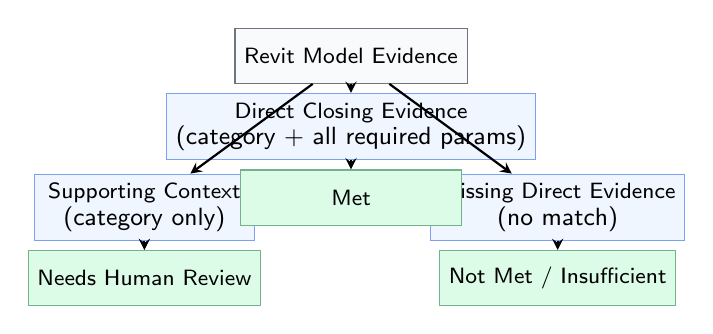
\begin{tikzpicture}[node distance=0.6cm and 0.3cm, auto]
\node[etype] (source) {Revit Model Evidence};
\node[eclass, below of=source, yshift=-0.3cm] (direct) {Direct Closing Evidence \\
  \small (category + all required params)};
\node[eclass, below left of=direct, xshift=-2.2cm, yshift=-0.6cm] (support)
  {Supporting Context \\
  \small (category only)};
\node[eclass, below right of=direct, xshift=2.2cm, yshift=-0.6cm] (miss)
  {Missing Direct Evidence \\
  \small (no match)};
\node[result, below of=support, yshift=-0.3cm] (sresult) {Needs Human Review};
\node[result, below of=direct, yshift=-0.3cm] (dresult) {Met};
\node[result, below of=miss, yshift=-0.3cm] (mresult) {Not Met / Insufficient};

\draw[arrow] (source) -- (direct);
\draw[arrow] (source) -- (support);
\draw[arrow] (source) -- (miss);
\draw[arrow] (direct) -- (dresult);
\draw[arrow] (support) -- (sresult);
\draw[arrow] (miss) -- (mresult);
\end{tikzpicture}
\end{tcolorbox}

% ============================================================
% 7. Status Logic
% ============================================================
\section{Status Logic}

Each requirement receives a final status after evaluating compliance, evidence, and actionability.

\subsection{Status Definitions}

\begin{longtable}{p{1.0in}p{2.2in}p{3.5in}}
\caption{Status definitions with conditions}
\label{tab:status-defs}\\
\toprule
\textbf{Status} & \textbf{Meaning} & \textbf{Condition} \\
\midrule
\endhead
Met & Requirement is satisfied. & Direct closing evidence found: element category matches,
  required parameters populated, evidence accepted. \\
Not Met & Requirement is not satisfied. & Element found but required parameters missing;
  or candidate evidence rejected; or non-compliant status set by reviewer. \\
Needs Human Review & System cannot determine status. Human judgment required.
  & Only supporting context found; evidence is candidate; validation type is
  Hybrid, Spec, or Manual; reviewer set needs\_review. \\
Insufficient Model Data & Required evidence not available in current export. & No matching element
  category; or data known to be outside Revit scope. \\
Not Applicable & Outside project scope or not actionable. & Non-actionable requirement;
  discipline/scope mismatch; or explicitly excluded. \\
\bottomrule
\end{longtable}

\subsection{Decision Table}

\begin{longtable}{p{1.6in}p{1.8in}p{1.0in}p{2.3in}}
\caption{Evidence situations and resulting status}
\label{tab:status-decision}\\
\toprule
\textbf{Condition} & \textbf{Evidence Situation} & \textbf{Status} & \textbf{Reasoning} \\
\midrule
\endhead
Direct panel and circuit evidence found & Element category + Panel + Circuit Number populated
  & Met & Direct closing evidence confirms fulfilment. \\
Element found, parameter missing & Element category matches; required parameter is empty
  & Not Met or Review & Missing = Not Met for model-checkable;
  Review for hybrid types. \\
Only supporting context & Element category matches but evidence is candidate / unreviewed
  & Needs Human Review & System cannot self-approve candidates. \\
Required evidence not exported & No elements of expected category in export & Insufficient
  Model Data & Data gap outside system control. \\
Outside project scope & Discipline or category mismatch & Not Applicable & Correctly scoped out. \\
Spec requirement with model hints & Model element type suggests but does not confirm
  & Needs Human Review & Spec validation requires human review regardless. \\
Reviewer rejection & Reviewer set status to ``rejected'' & Not Met & Human override respected. \\
Reviewer acceptance & Reviewer set status to ``accepted'' & Met & Human override respected. \\
Stale evidence & Evidence evaluated\_at $<$ latest export completed\_at & Pending review
  & Stale evidence flagged for re-evaluation. \\
\bottomrule
\end{longtable}

\subsection{Status Priority Chain}

The status evaluation follows a priority chain:

\begin{enumerate}
  \item Not actionable $\rightarrow$ \textsc{Not Applicable}.
  \item Compliance record exists $\rightarrow$ use its status (human override).
  \item No evidence row $\rightarrow$ \textsc{Missing}.
  \item Evidence accepted $\rightarrow$ \textsc{Met}.
  \item Evidence is candidate or needs review $\rightarrow$ \textsc{Needs Human Review}.
  \item Evidence rejected $\rightarrow$ \textsc{Not Met}.
  \item Fallback to evidence status: covered $\rightarrow$ \textsc{Met};
        needs\_review $\rightarrow$ \textsc{Needs Human Review};
        not\_applicable $\rightarrow$ \textsc{Not Applicable}.
  \item Default $\rightarrow$ \textsc{Missing}.
\end{enumerate}

% ============================================================
% Requirement Review Flow Diagram
% ============================================================
\section{Requirement Review Flow}

\vspace{-\parskip}
\begin{tcolorbox}[colback=white]
\centering
\small
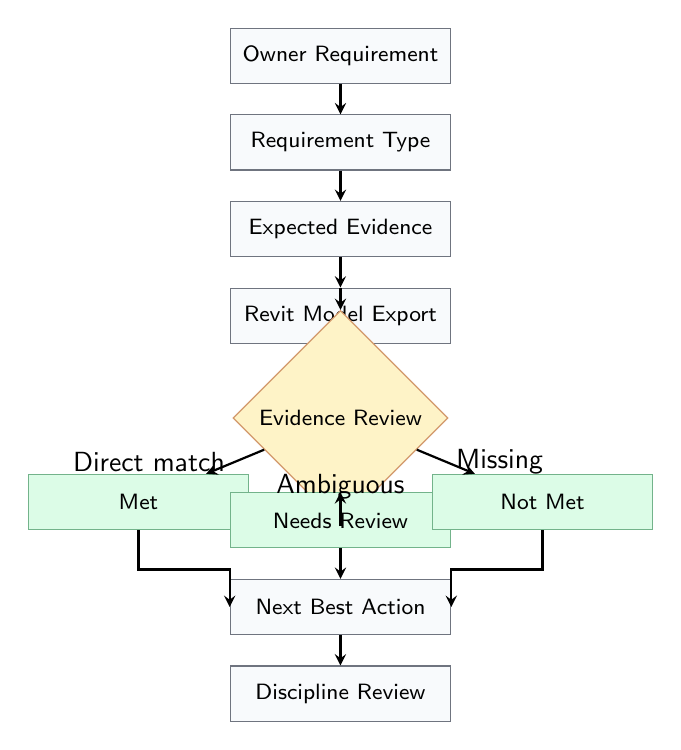
\begin{tikzpicture}[node distance=0.8cm and 0.3cm, auto]
\node[block] (req) {Owner Requirement};
\node[block, below of=req, yshift=-0.3cm] (type) {Requirement Type};
\node[block, below of=type, yshift=-0.3cm] (evidence) {Expected Evidence};
\node[block, below of=evidence, yshift=-0.3cm] (revit) {Revit Model Export};
\node[decision, below of=revit, yshift=-0.5cm] (eval) {Evidence Review};
\node[result, below left of=eval, xshift=-2.0cm, yshift=-0.5cm] (met) {Met};
\node[result, below of=eval, yshift=-0.5cm] (review) {Needs Review};
\node[result, below right of=eval, xshift=2.0cm, yshift=-0.5cm] (notmet) {Not Met};
\node[block, below of=review, yshift=-0.3cm] (action) {Next Best Action};
\node[block, below of=action, yshift=-0.3cm] (discipline) {Discipline Review};

\draw[arrow] (req) -- (type);
\draw[arrow] (type) -- (evidence);
\draw[arrow] (evidence) -- (revit);
\draw[arrow] (revit) -- (eval);
\draw[arrow] (eval) -- node[left] {Direct match} (met);
\draw[arrow] (eval) -- node[above] {Ambiguous} (review);
\draw[arrow] (eval) -- node[right] {Missing} (notmet);
\draw[arrow] (met.south) -- ++(0,-0.5cm) -| (action.west);
\draw[arrow] (review) -- (action);
\draw[arrow] (notmet.south) -- ++(0,-0.5cm) -| (action.east);
\draw[arrow] (action) -- (discipline);
\end{tikzpicture}
\end{tcolorbox}

% ============================================================
% 8. Key Issue Score
% ============================================================
\section{Key Issue Score}

The Key Issue Score is a prioritisation score, not a compliance score. It helps discipline leads
focus on the most important review items first.

\guardrailbox{\strong{Key Issue Score is a prioritisation score, not a compliance score.} It does
  not measure how many requirements are met; it ranks individual issues by their expected impact on
  deliverable readiness, actionability, and evidence gap severity.}

\subsection{Formula}

\[
\begin{aligned}
\text{KeyIssueScore} =\;& 0.25 \times \text{StatusSeverity}
+ 0.20 \times \text{DeliverableImpact} \\
&+ 0.20 \times \text{Actionability}
+ 0.15 \times \text{EvidenceGap} \\
&+ 0.10 \times \text{RequirementTypeRisk}
+ 0.10 \times \text{ImpactScale}
\end{aligned}
\]

\subsection{Weight Table}

\begin{longtable}{p{1.5in}p{0.7in}p{3.8in}}
\caption{Key Issue Score factors and their rationale\label{tab:key-issue-weights}}\\
\toprule
\textbf{Factor} & \textbf{Weight} & \textbf{Explanation} \\
\midrule
\endhead
Status Severity & 25\% & Not Met ranks highest, followed by Insufficient Model Data and Needs
  Human Review. Met contributes zero. \\
Deliverable Impact & 20\% & Items that can block DD/CD readiness, coordination deliverables, or
  milestone sign-off rank above minor documentation gaps. \\
Actionability & 20\% & Issues with a clear next step are easier to route and resolve. \\
Evidence Gap & 15\% & Missing equipment, missing parameters, or incomplete evidence raises
  priority. Items with no evidence score higher than partial evidence. \\
Requirement Type Risk & 10\% & Specification, drawing, and hybrid requirements carry higher
  inherent risk because they cannot be closed from model data alone. \\
Impact Scale & 10\% & Requirements affecting multiple elements, disciplines, or systems score
  higher than isolated single-element items. \\
\bottomrule
\end{longtable}

\subsection{Score Interpretation}

\begin{longtable}{p{0.9in}p{4.8in}}
\caption{Key Issue Score interpretation}
\label{tab:key-issue-interp}\\
\toprule
\textbf{Score Range} & \textbf{Meaning} \\
\midrule
\endhead
0.80 -- 1.00 & Critical --- likely blocker; immediate engineering attention recommended. \\
0.60 -- 0.79 & High --- significant risk; assign and resolve before next deliverable review. \\
0.40 -- 0.59 & Medium --- noteworthy gap; plan resolution in current review cycle. \\
0.00 -- 0.39 & Low --- minor or informational; address during normal QA/QC. \\
\bottomrule
\end{longtable}

\subsection{How It Helps Discipline Leads}

The Key Issue Score replaces an undifferentiated list of open items with a ranked, prioritised
action list. A discipline lead reviewing 100 requirements can immediately see:

\begin{itemize}
  \item Which 3--5 items are critical blockers (score $> 0.80$).
  \item Which items have clear next steps (high actionability) vs.\ items requiring scoping (low
        actionability).
  \item Which gaps are driven by missing model data (fixable in Revit) vs.\ requirements that
        inherently need drawing or spec review.
\end{itemize}

\subsection{Tuning the Score}

Weights are configurable through EMA feedback. If certain factors prove more important for a given
project or programme, the weighting can be adjusted. See Section~\ref{sec:tuning} (Tuning With EMA)
for details.

% ============================================================
% 9. Next Best Action Logic
% ============================================================
\section{Next Best Action Logic}

Each requirement that is not fully met receives a recommended next best action. The action is
generated based on the gap condition:

\begin{itemize}
  \item \textbf{No evidence:} ``Link evidence'' or ``Run sync''.
  \item \textbf{Validation type is spec/drawing/hybrid:} ``Review evidence'' or ``Review requirement''.
  \item \textbf{Status is Not Met:} ``Link evidence'' or ``Review requirement''.
  \item \textbf{Status is Needs Human Review:} ``Review requirement''.
  \item \textbf{Discipline unmapped:} ``Assign discipline''.
  \item \textbf{Requirement type is spec/manual:} ``Map evidence type''.
  \item \textbf{Evidence is candidate only:} ``Review evidence''.
  \item \textbf{Milestone not mapped:} ``Map milestone''.
\end{itemize}

\subsection{Action Types}

\begin{longtable}{p{1.5in}p{1.3in}p{3.5in}}
\caption{Next best action types and generation conditions}
\label{tab:next-actions}\\
\toprule
\textbf{Action Type} & \textbf{Label} & \textbf{When Generated} \\
\midrule
\endhead
link\_evidence & Link evidence & Requirement has no linked model, sheet, spec, or manual evidence. \\
review\_evidence & Review evidence & Evidence exists but is stale, candidate-only, or needs
  confirmation. \\
review\_requirement & Review requirement & Evidence exists but needs reviewer confirmation or
  clarification. \\
evaluate\_requirements & Evaluate requirements & Requirements not yet evaluated for the current
  deliverable. \\
assign\_discipline & Assign discipline & Requirement is missing a usable discipline mapping. \\
map\_milestone & Map milestone & Requirement not mapped to a DD/CD milestone. \\
map\_trade & Map trade & Requirement cannot contribute to trade readiness until a trade is assigned. \\
map\_evidence\_type & Map evidence type & Requirement not mapped to an expected evidence type. \\
attach\_source & Attach source & Requirement is missing a source file or owner resource reference. \\
run\_sync & Run sync & No completed sync exists; or latest sync is stale. \\
review\_trade\_gaps & Review trade gaps & Trade has unevaluated requirements and high/critical
  issues. \\
review\_issue\_backlog & Review issue backlog & High/critical issues exist without active owner
  requirements. \\
\bottomrule
\end{longtable}

\subsection{Examples}

\begin{longtable}{p{2.4in}p{4.8in}}
\caption{Next best action examples}
\label{tab:next-action-examples}\\
\toprule
\textbf{Situation} & \textbf{Next Best Action} \\
\midrule
\endhead
Panel/circuit parameter missing on lighting fixture. & Assign or verify panel and circuit values for
  affected lighting fixtures, then rerun the compliance check. \\
Manufacturer/spec requirement with no spec evidence linked. & Verify manufacturer/model against
  specifications. Attach or reference supporting spec section evidence. \\
Plumbing pipe requirement with hints but no connection evidence. & Confirm required pipe size and
  connection evidence. Review specification for material and detail requirements. \\
Drawing requirement with no sheet reference. & Review drawing/spec because model evidence alone is
  insufficient. Attach sheet reference or manual review annotation. \\
Technology device with no matching category in export. & Confirm whether devices are modelled,
  specified, or tracked outside Revit. Add family names or parameters if modelled. \\
Candidate evidence not yet reviewed. & Review candidate evidence. Accept if correct, reject if
  incorrect, or mark needs review for further investigation. \\
Stale sync. & Run a fresh Revit export and sync to update evidence. \\
Unmapped discipline. & Assign discipline mapping to enable trade readiness tracking. \\
\bottomrule
\end{longtable}

% ============================================================
% 10. Readiness and Report Relationship
% ============================================================
\section{Readiness and Report Relationship}

The Owner Requirements Report operates at three levels:

\begin{enumerate}
  \item \textbf{Requirement-level status:} Individual Met / Not Met / Needs Human Review per
        requirement. This is the atomic unit.
  \item \textbf{Trade (Discipline) Readiness:} Aggregated coverage by discipline, adjusted for open
        high/critical issues:
        \[
        \text{TradeReadiness} = \max\bigl(0,\;
        \text{Coverage} - (\text{Critical} \times 5.0 + \text{High} \times 2.0)\bigr)
        \]
  \item \textbf{Project Readiness:} A weighted composite:
        \[
        \text{OverallReadiness} = 0.50 \times \text{ReqCoverage}
        + 0.30 \times \text{QAQCHealth}
        + 0.20 \times \text{SyncFreshness}
        \]
\end{enumerate}

\subsection{Readiness Labels}

\begin{longtable}{p{0.9in}p{1.5in}p{3.2in}}
\caption{Readiness score labels and meanings}
\label{tab:readiness-labels}\\
\toprule
\textbf{Score} & \textbf{Label} & \textbf{Meaning} \\
\midrule
$\ge 90$ & Ready & All dimensions strong; minimal risk. \\
$\ge 75$ & On Track & Acceptable with minor gaps. \\
$\ge 60$ & At Risk & Notable gaps in one or more dimensions. \\
$\ge 40$ & Behind & Significant gaps requiring attention. \\
$< 40$ & Critical & Major blockers or missing data. \\
\bottomrule
\end{longtable}

\subsection{Readiness Components}

\begin{longtable}{p{1.5in}p{0.6in}p{4.0in}}
\caption{Readiness component formulas}
\label{tab:readiness-components}\\
\toprule
\textbf{Component} & \textbf{Weight} & \textbf{Formula} \\
\midrule
\endhead
Requirement Coverage & 50\% & (covered / applicable) $\times 100$ where covered = actionable
  requirements with compliant status and applicable excludes not\_applicable. \\
QA/QC Health & 30\% & $100 - (\text{penalty} / \max(\text{elements}/100, 1))$ where penalty =
  critical $\times 5.0 +$ high $\times 2.0 +$ medium $\times 0.75 +$ low $\times 0.25$. \\
Sync Freshness & 20\% & $\le 1$ day = 100; $\le 3$ days = 85; $\le 7$ days = 70;
  $\le 14$ days = 50; else = 25; None = 0. \\
\bottomrule
\end{longtable}

% ============================================================
% 11. Report Output Structure
% ============================================================
\section{Report Output Structure}

The generated report (HTML or PDF) is organised into the following sections:

\begin{longtable}{p{1.3in}p{1.6in}p{1.4in}p{2.0in}}
\caption{Report sections and reviewer actions}
\label{tab:report-sections}\\
\toprule
\textbf{Section} & \textbf{Purpose} & \textbf{Key Data} & \textbf{Reviewer Action} \\
\midrule
\endhead
Summary & KPI overview: total count, Met, Not Met, Needs Review, overall score, readiness label.
  & Score, label, counts, discipline breakdown & Identify concentration of risk. \\
Requirements & Full requirement register with status, evidence, and score per row.
  & ID, discipline, text, status, evidence, score & Review Met items for false positives. \\
Evidence & Evidence traceability: which elements and parameters support each requirement.
  & Evidence type, source ref, review status, matched params & Validate candidate evidence before
  accepting. \\
Elements & Referenced model element records. & Unique ID, category, family, type, level, key params
  & Verify element identification and parameter accuracy. \\
Rules & Rules applied to each requirement: classification, scoring, validation type.
  & Rule code, intent type, weight, match details & Understand status assignments. \\
Exports & Sync metadata. & Export ID, date, element count, status & Confirm data freshness. \\
Ask EMA AI & Chat interface grounded on report context. & Question input, AI response with
  references & Ask for explanations of statuses or evidence. \\
Taxonomy Matrix & Requirement type classification: expected categories, params, closeable flag.
  & Category, validation type, closeable, false-positive risk & Tune classification rules. \\
AI Audit & Deterministic rule trace log for each evaluated requirement.
  & Rule, input, match result, score contribution & Audit unexpected status assignments. \\
\bottomrule
\end{longtable}

\subsection{Hidden Report Context / JSON Source of Truth}

Self-contained HTML reports embed a hidden JSON context inside a
\code{<script type="application/json" id="ema-ai-report-context">} tag. This context serves as the
structured data source for both the visual report and the Ask EMA AI assistant.

\vspace{4pt}
\begin{tcolorbox}[colback=emaSoft2]
\small
\strong{JSON schema structure:}
\begin{itemize}
  \item \code{schema\_version} --- Version identifier for the context schema.
  \item \code{report\_metadata} --- Project name, date, generation timestamp, report hash.
  \item \code{summary} --- Counts (total, covered, missing, needs\_review, not\_applicable),
        coverage ratio, overall score, readiness label.
  \item \code{key\_issues} --- Ranked list with score, severity, requirement reference, and
        recommendation.
  \item \code{requirement\_results} --- Full per-requirement detail: data, evidence, status, score,
        next action.
  \item \code{ai\_lookup\_hints} --- Color mappings, anchor IDs, section ordering for the AI
        assistant.
  \item \code{evidence\_rows} --- Individual evidence records with type, status, source reference,
        confidence.
  \item \code{element\_records} --- Referenced element unique IDs, categories, family, type, level.
  \item \code{rules\_applied} --- Rule codes, classifications, scoring breakdowns per requirement.
  \item \code{next\_actions} --- Aggregated recommended actions with severity and owner routing.
\end{itemize}
\end{tcolorbox}

\guardrailbox{\strong{Ask EMA AI should ground answers on this report context and cite row numbers
  and requirement IDs.} The assistant must not invent evidence, element IDs, parameter values, or
  source rows not present in the loaded context.}

% ============================================================
% 12. Ask EMA AI / RAG Guardrails
% ============================================================
\section{Ask EMA AI / RAG Guardrails}

When the report includes an Ask EMA AI assistant, the following guardrails apply:

\begin{enumerate}
  \item \textbf{Model selector:} Users may choose between local (Ollama) and cloud (OpenAI-compatible)
        model providers.
  \item \textbf{Local vs.\ cloud distinction:} Local models run on the user's infrastructure and do
        not send data externally. Cloud models may send queries to a third-party API.
  \item \textbf{Local model privacy:} When using a local model, all report context remains on the
        local machine. No data leaves the deployment boundary.
  \item \textbf{Deterministic fallback:} If the AI model is unavailable or returns an unsafe
        response, the system falls back to a deterministic response template.
  \item \textbf{Answer grounding:} The assistant must answer based on the loaded report context
        JSON. It must not invent requirements, evidence, element IDs, or parameter values.
  \item \textbf{References:} The assistant should cite requirement IDs (e.g., REQ-E-042), evidence
        source references, and row numbers when explaining statuses.
  \item \textbf{Missing evidence language:} When asked about a missing item, the assistant should
        say ``No evidence found in the current report context'' rather than inventing an explanation.
  \item \textbf{No hallucinated compliance:} The assistant must not claim compliance, certification,
        or approval. It reports only what the loaded context contains.
\end{enumerate}

\guardrailbox{\textbf{Ask EMA AI can explain the loaded report context, but it does not create final
  engineering approval.}}

% ============================================================
% 13. AI Audit and Taxonomy Matrix
% ============================================================
\section{AI Audit and Taxonomy Matrix}

The taxonomy matrix documents the requirement type classification rules, expected categories,
expected parameters, exclusions, and false-positive risks.

\subsection{Taxonomy Matrix}

\begin{longtable}{p{1.1in}p{1.2in}p{1.2in}p{0.9in}p{1.3in}}
\caption{Taxonomy matrix: intent type, expected data, and risks}
\label{tab:taxonomy}\\
\toprule
\textbf{Intent Type} & \textbf{Expected Categories} & \textbf{Required Params} & \textbf{Model-Closeable?} & \textbf{False-Positive Risk} \\
\midrule
\endhead
technology & Communication, Data, Fire Alarm, Security, Nurse Call, Telephone Devices & Mark,
  System Name & Partial & Generic ``device'' may match non-target categories \\
mechanical & Mechanical Equipment & Mark, Type Mark & Partial & ``Equipment'' broadly matches
  mechanical categories \\
lighting & Lighting Fixtures & Panel, Circuit Number & Yes, if params populated
  & ``Light'' or ``luminaire'' in family names may produce false matches \\
plumbing & Plumbing Fixtures, Pipes, Fittings, Accessories & Mark, Type Mark & Partial
  & ``Pipe'' broadly matches; connection evidence requires param checks \\
electrical\_panel & Electrical Equipment & Supply From & Yes
  & ``Panel'' excluded from keywords; only terms like ``panelboard'' match \\
electrical\_fixture & Electrical Fixtures & Panel, Circuit Number & Yes, if params populated
  & ``Power'' or ``plug'' may match broadly; circuit presence reduces false positives \\
generic\_model & (none) & (none) & No & Fallback for unmatched requirements; risks false Met if
  category alone treated as evidence \\
\bottomrule
\end{longtable}

\subsection{Why This Matters}

\begin{itemize}
  \item \textbf{Reduces false Met:} Parameter-level validation prevents marking a requirement Met
        simply because an element of the right category exists.
  \item \textbf{Separates evidence from context:} Contextual clues (family name, type name, level)
        contribute to scoring but do not independently close requirements.
  \item \textbf{Candidate scope warnings:} Requirements classified as \code{generic\_model} have no
        expected categories or parameters and always require human review.
  \item \textbf{Narrative contradiction checks:} Conflicting review statuses on the same requirement
        are flagged.
  \item \textbf{Generic next action detection:} Overly generic actions on high-scored issues suggest
        further tuning of classification rules.
\end{itemize}

\subsection{Excluded Categories}

The following categories are excluded from evidence matching because their presence alone does not
provide meaningful evidence:
\begin{itemize}
  \item Generic annotation categories (Text Notes, Dimensions, Detail Items).
  \item View-specific categories (View Titles, Revisions, Sheet Titles).
  \item Non-physical categories (Project Information, Shared Parameters).
\end{itemize}

\subsection{Parameter Validation Rules}

For each model-checkable requirement, the system validates:
\begin{itemize}
  \item Parameter presence: The parameter must exist on the element.
  \item Non-emptiness: The value must be a non-empty string after stripping whitespace.
  \item Relevance: The parameter must be among the required parameters for the intent pattern.
\end{itemize}

\subsection{Narrative Checks}

The system performs basic narrative consistency checks:
\begin{itemize}
  \item Evidence accepted but evidence type is ``candidate'' $\rightarrow$ flag inconsistency.
  \item Requirement non-compliant but has accepted evidence $\rightarrow$ flag conflict.
  \item Multiple evidence records with contradictory review statuses $\rightarrow$ flag for
        resolution.
\end{itemize}

% ============================================================
% 14. Tuning With EMA
% ============================================================
\section{Tuning With EMA}
\label{sec:tuning}

EMA can tune the following aspects of the report logic:

\begin{longtable}{p{1.8in}p{4.5in}}
\caption{Tunable parameters}
\label{tab:tunable}\\
\toprule
\textbf{Parameter} & \textbf{Description} \\
\midrule
\endhead
Scoring weights & Adjust Key Issue Score component weights: Status Severity, Deliverable Impact,
  Actionability, Evidence Gap, Requirement Type Risk, Impact Scale. \\
Requirement type priorities & Reorder or reclassify requirement families (Model, Hybrid,
  Specification, Drawing, Manual). \\
Expected evidence & Add or remove expected categories, keywords, and required parameters per
  intent pattern. \\
Status thresholds & Adjust score thresholds at which statuses are assigned. \\
Discipline-specific rules & Create custom classification rules for specific disciplines. \\
Model-closeable flags & Reclassify requirement types as model-closeable or not. \\
Review feedback loops & Capture accept/reject decisions to improve candidate evidence matching. \\
Excluded categories & Add or remove Revit categories from evidence matching. \\
\bottomrule
\end{longtable}

\subsection{Tuning Loop}

\vspace{-\parskip}
\begin{tcolorbox}[colback=white]
\centering
\small
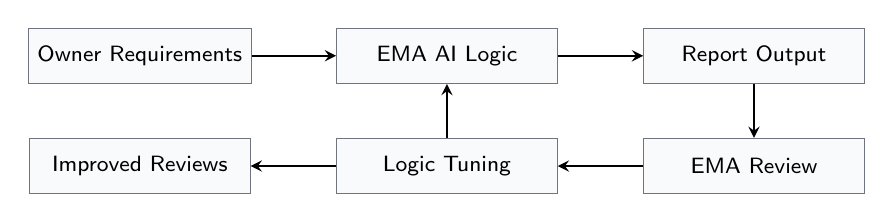
\begin{tikzpicture}[node distance=0.7cm and 0.3cm, auto]
\node[loopblock] (or) {Owner Requirements};
\node[loopblock, right of=or, xshift=3.2cm] (log) {EMA AI Logic};
\node[loopblock, right of=log, xshift=3.2cm] (out) {Report Output};
\node[loopblock, below of=out, yshift=-0.7cm] (rev) {EMA Review};
\node[loopblock, below of=log, yshift=-0.7cm] (tune) {Logic Tuning};
\node[loopblock, below of=or, yshift=-0.7cm] (imp) {Improved Reviews};

\draw[arrow] (or) -- (log);
\draw[arrow] (log) -- (out);
\draw[arrow] (out) -- (rev);
\draw[arrow] (rev) -- (tune);
\draw[arrow] (tune) -- (log);
\draw[arrow] (tune) -- (imp);
\end{tikzpicture}

\vspace{4pt}
\muted{Review $\rightarrow$ Tune $\rightarrow$ Improve: the iterative feedback cycle.}
\end{tcolorbox}

\keyconcept{\strong{Feedback mechanism:} Reviewers can accept, reject, or flag candidate evidence
  through the API or UI. These decisions are persisted and can be used to tune classification rules,
  parameter requirements, and scoring weights. Over multiple review cycles, the system improves its
  matching accuracy and reduces false positives.}

% ============================================================
% 15. Customer-Facing Guardrails
% ============================================================
\section{Customer-Facing Guardrails}

The following principles govern every report and every AI interaction. They are designed to ensure
that EMA AI remains a supportive tool for engineering review, never a substitute for professional
judgment.

\guardrailbox{\strong{1. EMA AI is not a final compliance certification.} The report is a structured
  first-pass evidence review. It does not certify code compliance, contract compliance, or
  professional approval.}

\guardrailbox{\strong{2. EMA AI does not replace licensed engineering review.} Final validation
  remains subject to engineering review, drawings, specifications, and owner acceptance.}

\guardrailbox{\strong{3. EMA AI does not treat generic model presence as proof.} Category, family,
  type, or level alone should not close high-risk requirements unless the requirement type explicitly
  allows it.}

\guardrailbox{\strong{4. EMA AI escalates ambiguous, spec, and manual requirements to human review.}
  Requirements that cannot be fully evaluated from model evidence are marked
  \textsc{Needs Human Review}.}

\guardrailbox{\strong{5. EMA AI separates direct evidence from supporting context.} Direct Closing
  Evidence can close a requirement. Supporting Context suggests relevance but requires human review
  before acceptance.}

\guardrailbox{\strong{6. EMA AI can be tuned with EMA standards and reviewer feedback.} Scoring
  weights, requirement priorities, expected evidence, and status thresholds are configurable through
  EMA feedback (see Section~\ref{sec:tuning}).}

\guardrailbox{\strong{7. EMA AI is traceable and auditable.} Every status decision traces to
  specific evidence rows, rule codes, requirement IDs, and scoring breakdowns. The system maintains a
  complete audit trail.}

\guardrailbox{\strong{8. EMA AI does not provide legal, contractual, or code-compliance opinions.}
  All outputs must be reviewed by qualified professionals before any deliverable sign-off.}

% ============================================================
% Appendix A: Glossary
% ============================================================
\clearpage
\appendix
\section{Appendix A --- Glossary}

\begin{longtable}{p{1.6in}p{5.0in}}
\caption{Glossary of key terms}
\label{tab:glossary}\\
\toprule
\textbf{Term} & \textbf{Definition} \\
\midrule
\endhead
Owner Requirement & A client-supplied statement of expected project outcome or deliverable condition,
  typically from an Excel workbook. The atomic unit of the report. \\
Requirement Type & Classification into Model-Checkable, Hybrid, Specification, Drawing/Manual, or
  Ambiguous based on validation approach. \\
Validation Type & The type of evidence needed: Model, Drawing, Specification, Manual, Hybrid, or Not
  Model-Closeable. \\
Direct Closing Evidence & Evidence that conclusively satisfies a requirement: matching element
  category plus all required parameters populated with meaningful values. \\
Supporting Context & Evidence suggesting relevance but not confirming: matching category but missing
  one or more required parameters. Requires human review. \\
Missing Direct Evidence & No element of the expected category found, or no parameter values
  populated. \\
Evidence Gap & The difference between expected and available evidence. May be partial (missing
  parameter) or total (no evidence at all). \\
Key Issue Score & A prioritisation score (0.00--1.00) ranking individual issues by expected impact
  on deliverable readiness. Not a compliance score. \\
Readiness & A composite score (0--100) weighted across requirement coverage (50\%), QA/QC health
  (30\%), and sync freshness (20\%). \\
Next Best Action & A recommended action for a requirement that is not fully met, generated from
  evidence, validation type, status, and discipline conditions. \\
Candidate Scope & Evidence meeting the minimum scoring threshold ($\ge 0.40$) but not yet reviewed by
  a human. Must not count as proof. \\
Human-in-the-loop & A design principle requiring human review for any status decision that cannot be
  fully supported by deterministic model evidence. \\
Model-closeable & A requirement whose satisfaction can be fully determined from Revit model data
  alone (category plus parameter values). \\
Hybrid Requirement & A requirement with a model-checkable component (device presence) plus an
  additional drawing, spec, or manual evidence requirement. \\
\bottomrule
\end{longtable}

% ============================================================
% Appendix B: Example Requirement Evaluations
% ============================================================
\clearpage
\section{Appendix B --- Example Requirement Evaluations}

The following worked examples illustrate how the system evaluates requirements across different
validation types and evidence situations.

\subsection*{Example 1: Panel/Circuit Assignment (Model-Checkable)}

\begin{tcolorbox}[colback=white]
\begin{tabularx}{\textwidth}{p{1.4in}p{4.8in}}
\toprule
\smalllabel{Requirement Text} & Lighting fixtures shall be connected to panel and circuit
  information before the DD 30\% deliverable. \\
\smalllabel{Validation Type} & Model \\
\smalllabel{Expected Evidence} & Lighting Fixture element(s) with Panel and Circuit Number
  parameters populated. \\
\smalllabel{Available Evidence} & Lighting Fixture elements found. Panel = ``LP1'' populated on
  some instances; others have empty Circuit Number. \\
\smalllabel{Missing Evidence} & Circuit Number empty on 3 of 12 fixture instances. \\
\smalllabel{Status} & \notmetbadge \\
\smalllabel{Next Best Action} & Assign or verify panel and circuit values for affected lighting
  fixtures, then rerun the compliance check. \\
\smalllabel{Rationale} & Model-checkable with partial evidence. Missing parameter on subset drives
  Not Met. Score elevated due to DD 30\% milestone impact. \\
\bottomrule
\end{tabularx}
\end{tcolorbox}

\subsection*{Example 2: Manufacturer/Spec Requirement (Specification)}

\begin{tcolorbox}[colback=white]
\begin{tabularx}{\textwidth}{p{1.4in}p{4.8in}}
\toprule
\smalllabel{Requirement Text} & Sloan flush valves shall be provided at all water closets. \\
\smalllabel{Validation Type} & Specification \\
\smalllabel{Expected Evidence} & Spec section reference confirming Sloan flush valve standard;
  model evidence of water closet elements with relevant family names. \\
\smalllabel{Available Evidence} & Water closet elements found. Family name includes ``Sloan'' on
  some but not all instances. No spec section reference linked. \\
\smalllabel{Missing Evidence} & No confirmed spec section evidence. No manual review annotation for
  non-Sloan families. \\
\smalllabel{Status} & \reviewbadge \\
\smalllabel{Next Best Action} & Verify manufacturer and model against specifications. Attach or
  reference supporting spec section evidence. \\
\smalllabel{Rationale} & Specification type cannot be closed from model evidence alone. Family name
  suggests but does not confirm. Needs Human Review regardless of model hints. \\
\bottomrule
\end{tabularx}
\end{tcolorbox}

\subsection*{Example 3: Plumbing Connection Requirement (Hybrid)}

\begin{tcolorbox}[colback=white]
\begin{tabularx}{\textwidth}{p{1.4in}p{4.8in}}
\toprule
\smalllabel{Requirement Text} & Soap dispensers shall have a cold water connection. \\
\smalllabel{Validation Type} & Hybrid \\
\smalllabel{Expected Evidence} & Soap dispenser fixture element plus connection parameter or pipe
  adjacency plus spec or detail confirmation. \\
\smalllabel{Available Evidence} & Soap dispenser fixture elements found in Plumbing Fixtures
  category. No connection parameter populated. \\
\smalllabel{Missing Evidence} & No pipe adjacency data; no connection parameter; no spec section or
  detail reference. \\
\smalllabel{Status} & \reviewbadge \\
\smalllabel{Next Best Action} & Confirm required pipe size and connection evidence. Review
  specification for connection requirements. \\
\smalllabel{Rationale} & Hybrid type: fixture presence partially confirmable, but connection requires
  detail or spec review. Needs Human Review. \\
\bottomrule
\end{tabularx}
\end{tcolorbox}

\subsection*{Example 4: Mechanical Termination/Access Requirement (Hybrid)}

\begin{tcolorbox}[colback=white]
\begin{tabularx}{\textwidth}{p{1.4in}p{4.8in}}
\toprule
\smalllabel{Requirement Text} & Dryer vents shall terminate to the exterior with a backdraft damper.
\\
\smalllabel{Validation Type} & Hybrid \\
\smalllabel{Expected Evidence} & Mechanical equipment element plus termination point or connection to
  exterior plus detail or spec confirmation. \\
\smalllabel{Available Evidence} & Dryer vent cap family found in model. No exterior termination
  parameter; no backdraft damper parameter. \\
\smalllabel{Missing Evidence} & No exterior connection modelled; no backdraft damper parameter. \\
\smalllabel{Status} & \reviewbadge \\
\smalllabel{Next Best Action} & Verify termination detail against architectural drawings. Attach or
  reference sheet evidence for termination point. \\
\smalllabel{Rationale} & Hybrid type. Model evidence suggests device presence but cannot confirm
  termination method or damper inclusion. \\
\bottomrule
\end{tabularx}
\end{tcolorbox}

\subsection*{Example 5: Drawing/Manual Coordination Requirement (Drawing)}

\begin{tcolorbox}[colback=white]
\begin{tabularx}{\textwidth}{p{1.4in}p{4.8in}}
\toprule
\smalllabel{Requirement Text} & Conduit routing shall be coordinated with structural and
  architectural elements. \\
\smalllabel{Validation Type} & Drawing \\
\smalllabel{Expected Evidence} & Coordination sheet reference, clash detection report, or manual
  review annotation. \\
\smalllabel{Available Evidence} & Some conduit elements found in Electrical Fixtures category. No
  coordination sheet referenced. No clash detection evidence. \\
\smalllabel{Missing Evidence} & No drawing, sheet, or manual evidence confirming coordination review.
\\
\smalllabel{Status} & \insufficientbadge \\
\smalllabel{Next Best Action} & Review drawing/spec; model evidence alone is insufficient. Confirm
  coordination review status and attach sheet reference. \\
\smalllabel{Rationale} & Drawing type: conduit presence is only contextual. Full closure requires
  coordination review evidence. \\
\bottomrule
\end{tabularx}
\end{tcolorbox}

% ============================================================
% Document Notes
% ============================================================
\clearpage
\section*{Document Notes}

\begin{tcolorbox}[colback=white]
\small
\textbf{Document status:} This document describes the EMA AI Owner Requirements Report logic as
implemented in the MVP (June 2026). All descriptions reflect the current production codebase.
Weights, thresholds, and classification rules are subject to tuning based on EMA feedback and review
cycles.

\vspace{6pt}
\textbf{Limitations:}
\begin{itemize}
  \item The evidence resolver operates on exported Revit data only. Data not exported (linked model
        elements without parameters, unsupported categories) is invisible to the system.
  \item Specification and drawing requirements cannot be fully evaluated without linked spec sections
        or sheet references. Current MVP marks these as Needs Human Review.
  \item Intent classification uses keyword matching, not semantic understanding. Requirements with
        uncommon terminology may fall to the catch-all fallback.
  \item The Key Issue Score is a prioritisation heuristic and should be reviewed and tuned per
        project or programme.
\end{itemize}

\vspace{6pt}
\textbf{Report boundary:} This is a technical description of the EMA AI logic framework. It does not
constitute a compliance certification, engineering approval, or contractual document.

\vspace{6pt}
\textbf{Feedback loop:} The current logic provides a strong starting point. EMA feedback will tune
priority rules, confidence thresholds, and escalation criteria over the review cycle.
\end{tcolorbox}

\vfill
\begin{center}
\muted{--- End of Document ---}
\end{center}

\end{document}
